\documentclass[crop=false]{standalone}
% --- ПРЕАМБУЛА ДЛЯ ПОДДЕРЖКИ РУССКОГО ЯЗЫКА И МАТЕМАТИКИ ---
\usepackage[T2A]{fontenc}
\usepackage[utf8]{inputenc}
\usepackage[russian]{babel}
\usepackage{amsmath}
\usepackage{geometry}
\usepackage{amssymb}
\usepackage{graphicx}
\usepackage{float}
\usepackage{import}
\geometry{a4paper, top=2cm, bottom=2cm, left=2cm, right=2cm}
\newcommand{\sidecomment}[1]{\marginpar{\raggedright\scriptsize\itshape #1}}
\newcommand{\iu}{\mathrm{i}}

\newcommand{\Def}{%
    \text{Def}%
    \hspace{-0.85em}% Сдвиг назад ровно на середину (подберите под шрифт)
    \raisebox{0.1ex}{/}% Черта
    \hspace{1em}% Возврат к концу слова + небольшой отступ
}

\renewcommand{\Re}{\operatorname{Re}}
\renewcommand{\Im}{\operatorname{Im}}

\ifstandalone
    \newcommand{\lecturebreak}{} % В отдельном файле лекции разрыв не нужен
\else
    \newcommand{\lecturebreak}{\clearpage} % В полной книге - начинаем с новой страницы
\fi

\newcounter{lecturenumber} % Создаем счетчик для нумерации лекций
\newcommand{\lecture}[2]{
    \lecturebreak
    \refstepcounter{lecturenumber} % Увеличиваем счетчик на 1
    \par\vspace{2em}\noindent % Отступ сверху и убираем абзацный отступ
    {\Large\bfseries % Делаем заголовок крупным и жирным
    Лекция \thelecturenumber: #1 % Выводим "Лекция N: Тема"
    \hfill % Растягиваем пробел, чтобы дата была справа
    \large\textit{#2}} % Выводим дату курсивом
    \par\vspace{1em} % Небольшой отступ снизу
    \addcontentsline{toc}{section}{Лекция \thelecturenumber: #1} % Добавляем в оглавление
    \par
}

\newcommand{\TwoCols}[2]{%
  \par\noindent % Начать с новой строки без отступа
  \begin{minipage}[t]{0.48\textwidth}
    #1
  \end{minipage}% <-- Важный '%' для удаления пробела
  \hfill % Растягивающийся пробел между колонками
  \begin{minipage}[t]{0.48\textwidth}
    #2
  \end{minipage}% <-- Важный '%' для удаления пробела
  \par%
}

\pagestyle{plain} % Включаем нумерацию страниц\
\begin{document}
\lecture{}{25.05}
\section{Колебания систем с одной степенью свободы}
% fixme картинка в телефоне
\[T = \frac{m \dot \varphi^2 l^2}{2} \qquad \Pi = - m g l \cos \varphi \qquad L = \frac{m l^2 \dot \varphi^2}{2} + m g l \cos \varphi\]
\[m l^2 \ddot \varphi + m g l \sin \varphi = Q^*\]
\[Q^* = \frac{\delta A}{\delta \varphi} = \frac{- b^* \dot \varphi \delta \varphi}{\delta \varphi} \qquad m l^2 \ddot \varphi + m g l \sin \varphi = - b^* \dot \varphi\]
\[\ddot \varphi + \frac{b^*}{m l^2} \dot \varphi + \frac{g}{l} \varphi = 0 \qquad \ddot \varphi + 2 b \dot \varphi + \omega^2 \varphi = 0\]
Линейное уравнение малых свободных затухающих колебаний около положения равновесия

\noindent \keypoint При $2 b < 0$ система нефизична, при отрицательном коэффициенте при $\varphi$ равновесие неустойчиво

\noindent \keypoint 
\[\lambda_{1, 2} = - b \pm \sqrt{b^2 - \omega^2} \qquad \]
\[\begin{aligned}
&b > \omega \implies \varphi = C_1 e^{\lambda_1 t} + C_2 e^{\lambda_2 t} \qquad \lambda_1 , \lambda_2 < 0 \\
&b = \omega \implies \varphi = C_1 e^{-b t } + C_2 t e^{- b t} \\
& b < \omega \implies \varphi = C_1 \cos \lambda_1 t + C_2 \sin \lambda_2 t  = A e^{- b t} \cos\left( t \sqrt{\omega^2 - b^2} + \psi \right) \qquad \text{затухающее колебание} 
\end{aligned}
\]
где $A, \psi$ зависят от начальных условий

\noindent \keypoint Уравнение вынужденных колебаний
\[\ddot \varphi + 2 b \dot \varphi+ \omega^2 \varphi = A \sin(\omega_0 t + \psi_0) \quad b = 0\]
\[\ddot \varphi + \omega^2 \varphi = A \sin(\omega_0 t + \psi_0) \implies \varphi_{\text{частн}} = A_0 \sin (\omega_0 t + \psi_0)\]
\[- A_0 \omega_0^2 \sin(\omega_0 t + \psi_0) + \omega^2 A_0 \sin(\omega_0 t + \psi_0) = A \sin (\omega_0 t + \psi_0)\]
\[A_0 = \frac{A}{\omega^2 - \omega_0^2} \qquad \varphi = C \cos(\omega t + \psi) + \frac{A}{\omega^2 - \omega_0^2} \sin(\omega_0 t + \psi_0)\]
В резонансном случае $\omega = \omega_0$ модуль амплитуды колебаний будет увеличиваться(дифур по другому решается)
\[\varphi_{\text{частн}} = - \frac{A}{2 \omega_0} t \sin ( \omega_0 t + \psi_0)\]
Без диссипации, в резонансном случае амплитуда уходит в бесконечность, с диссипацией локальный максимум

\begin{figure}[H]
    \centering
    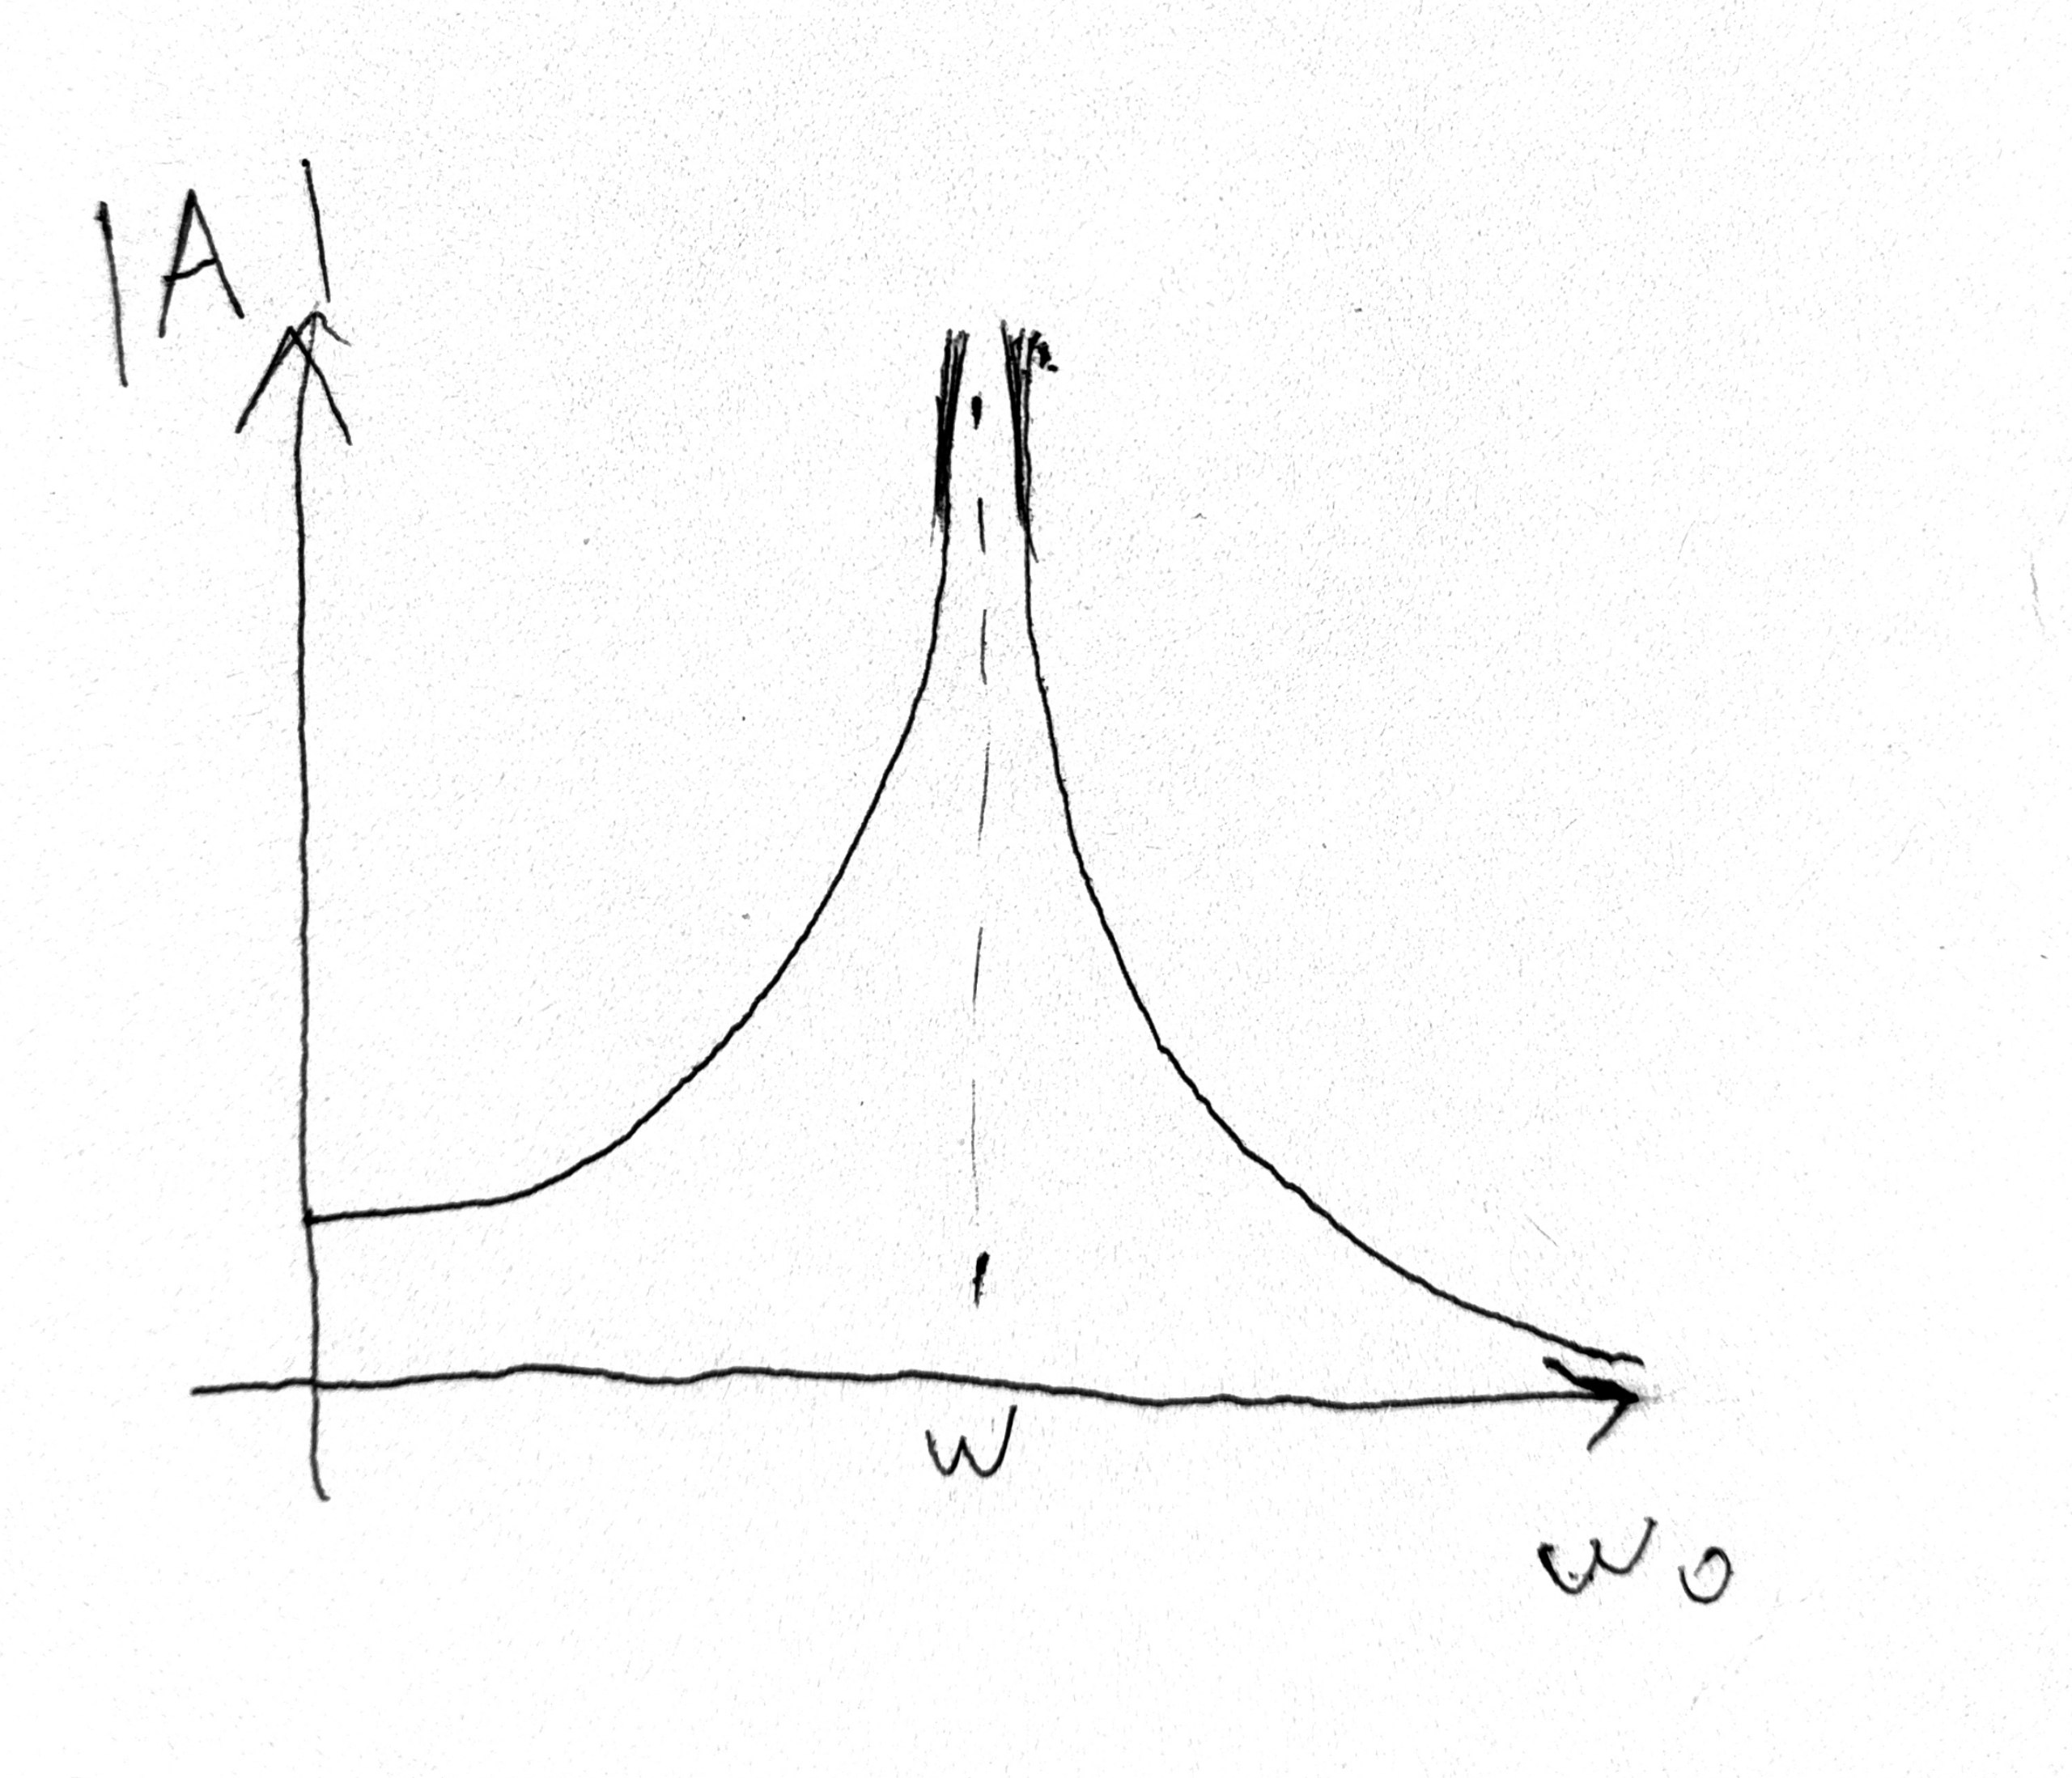
\includegraphics[width=0.35\textwidth]{b=0.jpg}
    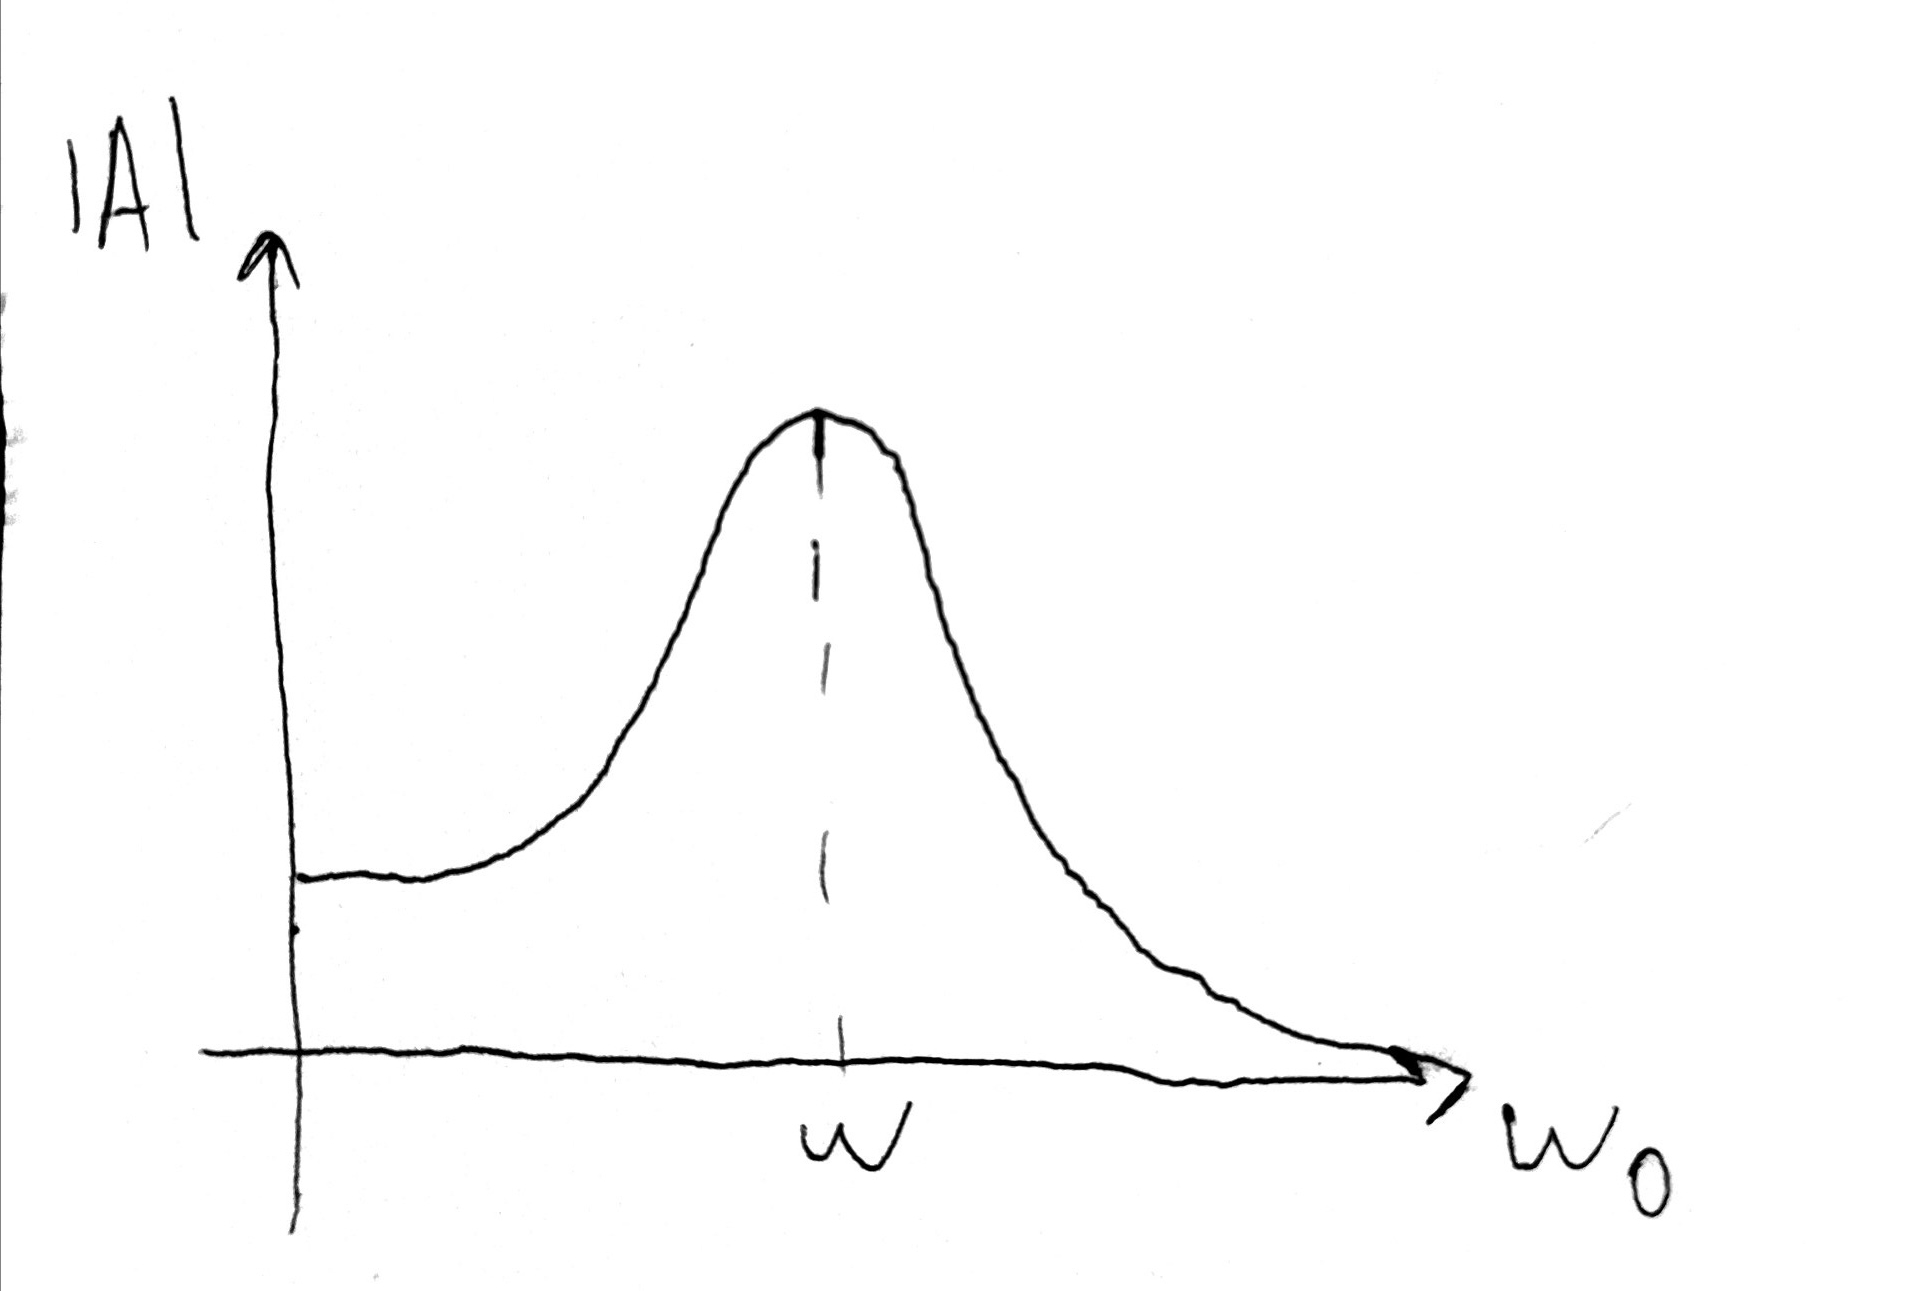
\includegraphics[width=0.35\textwidth]{bneq0.jpg}
    \caption{$b=0$ и $b\neq 0$}
    \label{fig:myimage} 
\end{figure}
Если разложить синус на большое число членов ряда, то получаем осциляттор Дуффинга
% fixme картинка кривой график в телефоне

\section{для нескольких степеней свободы}
\[\frac{d }{d t} \frac{\partial T}{\partial \dot q_i} - \frac{\partial T}{\partial q_i} = Q_i\]
сдвиг: положение равновесия в нуле фазового пространства, то есть $Q_i(0) =0$

\noindent \keypoint 

для склерономных систем

Уравнения Лагранжа имеют вид
\[A \ddot {\bar q }+ B \dot {\bar q} + (C + C^*) \bar q =0 \qquad A = (a_{i j}^0)\]
        \[ b_{i j} = - \left. \frac{\partial Q_i^*}{\partial \dot q_j} \right|_0 \qquad c_{i j} = \left. \frac{\partial^2 \Pi}{\partial q_i q_j}\right|_0 \quad c_{i j}^* = - \left.\frac{Q^*_i}{\partial q_j} \right|_0\]

\begin{proof}
    
    \[T = T_2 + \underbrace{T_1 + T_0}_0 = T_2 = \frac{1}{2} \sum_{i, j = 1}^n a_{i j} \dot q_i \dot q_j\]
    \[a_{i j}(q_1, \dots , q_n) \approx a_{i j}^0 + \sum_{l=1}^n \left. \frac{\partial a_{i j}}{\partial q_l} \right|_{0} q_l  \qquad a_{i j}^0 = \left.\frac{\partial^2 T_2}{\partial \dot q_j \partial \dot q_i}\right|_{0} \implies T_2 \approx \frac{1}{2} \sum_{i, j =1}^{n} a_{i j}^0 \dot q_i \dot q_j\]
    % fixme 0 из коорд пространства некрасиво написано
    \[
    Q_i = \frac{-\partial \Pi}{\partial q_i} + Q_i^* \qquad 
        \begin{aligned}
            Q_i(q, \dot q) &\approx Q_i(0, 0) + \sum_{j=1}^{n} \left. \frac{\partial Q_i}{\partial q_j} \right|_{0} q_j + \sum_{j=1}^{n}  \left. \frac{\partial Q_i}{\partial \dot q_j}\right|_{0} \dot q_j \\
            &= - \sum_{j=1}^{n} \left. \frac{\partial^2 \Pi}{\partial q_j \partial q_i} \right|_{0} q_j + \sum_{j=1}^{n} \left. \frac{\partial Q_i^*}{\partial q_j} \right|_{0} q_j + \sum_{j=1}^{n} \left. \frac{\partial Q_i^*}{\partial \dot q_j} \right|_0 \dot q_j \\
        \end{aligned}
        \]
        
        $c_{i j}$ — квази-упругие коэффициенты
        \[\frac{d}{d t} \sum_{j=1}^{n} a_{i j}^0 \dot q_j - 0 = \sum_{j=1}^{n} a_{i j}^0 \ddot q_j = Q_i \qquad \sum_{j=1}^{n} a_{i j}^0 \ddot q_j  + \sum_{j=1}^{n} c_{i j} q_j + \sum_{j=1}^{n} c^*_{i j} q_j + \sum_{j=1}^{n} b_{i j} \dot q_j = 0 \]
    \end{proof}
\noindent \keypoint

для консервативных систем

Существует такая замена, что системы эквивалентны
\[A \ddot{\bar q} + C \bar q = 0 \iff \ddot \theta_i + \lambda_i \theta_i = 0\]
\begin{proof}
    \[\bar q = U \bar \theta\]
    $A, C$ — задают квадратичные формы, $A$ надо перевести в единичную, $C$ в диагональную, $A$ положительно определена,  можно привести эти квадратичные формы одновременно к диагональному виду
    
    Сергей Алексеевич сказал, что квадратичные формы задают эллипсоиды, тогда:
    \begin{enumerate}
        \item поворот
        \item масштабирование
        \item поворот
    \end{enumerate}
    \[\bar q^T A q = \sum_{j=1}^{n} \theta_j^2 \qquad \bar q^T C \bar q = \sum_{j=1}^{n} \lambda_j \theta_j^2\]
\end{proof}
Замечание:
\[\theta_i = A_{i - 1} \sin(\sqrt \lambda_i t + \psi_{i-1})\]
\end{document}